
\documentclass{article}
\usepackage{amsmath}
\usepackage{hyperref}
\usepackage{enumerate}
\usepackage{listings}
\usepackage{graphicx}
\usepackage{rotating}
\graphicspath{ {../figures/} }
\begin{document}
\newcommand{\ihs}{\mathrm{arcsinh}}
\title{ML Techniques to Recover Treatment Effects from Karlan and List (2007) \\ HW1, Econ 293}
\author{Luis Armona\footnote{Coding done in colloboration with Jack Blundell} \\ \href{mailto:larmona@stanford.edu}{larmona@stanford.edu} }
\maketitle

\section{Setup}
Here, we investigate the treatment effect of offering any sort of ``match'' promise on charitable giving. Specifically, we look at Karlan \& List's 2007 AER paper : ``Does Price Matter in Charitable Giving? Evidence from a Large-Scale Natural Field Experiment'', which randomly selected 2/3 of the population of prior donors of a large charity to recieve one of nine treatments that were a variation of promising to match any donations for a limited time via an outside donor. The control group recieved a similar letter soliciting donations with no promise of a matching donation to theirs. \\ \indent
Our focus is on the average treatment effect (ATE) of promising to match donations on expected dollars donated in response to the solicitation. First, we recreate the average treatment effect documented in the paper. This is column (1) of Table 4 in the paper. We estimate an average treatment effect of an additional
\$0.1536 from the matching promise in the solicitation, consistent with the paper. The confidence interval is estimated to be $[-0.008,0.315]$.We then transform the paper's randomized experiment into an observational study by implementing a selection rule of the sample that depends on an interaction of treatment with baseline covariates of the donors. Specifically, let $K_i$ be an indicator for whether an individual is kept in the sample for the ``observational'' study, and let $\psi(X_i) = Pr(K_i=1|X_i)$ be the respondent's ``propensity'' to be kept in the sample. I define this differentially between donors depending on their assignment to treatment and control:
\[
  \psi(X_i)= \begin{cases}
  	  (.01 + -0.01*\ihs(X_{3,i})^5 + \ihs(X_{3,i})^3)/300 & \text{if $W_i=1$} \\
	  (X_{2,s}+1)*(\arccos(X_{1,s})*\arctan(X_{1,s}) )/3 & \text{if $W_i=0$} \\ 
     0.5 & \text{if missing one of $X_{1,s},X_{2,s},X_{3,i}$}
      \end{cases} 
\]
Where $W_i$ is a treatment indicator, $X_{3,i}$ is the highest previous donation by the donor, $X_{2,s}$ is the number of cases the charity undertook in the state $s$ from 2004-05, and $X_{2,s}$ is the state's voting share for George Bush in the 2004 presidential election, and $\ihs$ is the inverse hyperbolic sine function (e.g. $\ihs(X) = \log(X_{3,i} + \sqrt{X_{3,i} ^ 2 + 1}$). Figures \ref{dc} and \ref{dt} contain plots of this function for treatment/control groups.
So a treatment group individual's selection propbability is proportional to the inverse-hyperbolic sine (IHS) of their highest previous donation, while a control group individual's selection probability is proportional to a complex trigonometric function of state characteristics, specifically, the caseload of the organization in the state and their conservative ideological tendency, as measured by the bush vote share. Those with missing covariates are given 50-50 odds of being kept in the sample. 

From our selection rule, we can directly use Bayes' rule to back out the true propensity score for treatment, conditional on the covariates,$X_i$. for the non-random selected subsample. Specifically, the propensity score is:
\begin{align*}
\rho(X_i) = P(W_i=1|K_i=1) &= \frac{P(K_i=1|W_i=1)P(W_i=1) }{P(K_i=1|W_i=1)P(W_i=1) + P(K_i=1|W_i=0)P(W_i=0) } \\
 &= \frac{\psi(X_i|W_i=1)\frac{2}{3}}{ \psi(X_i|W_i=1)\frac{2}{3} + \psi(X_i|W_i=0)\frac{1}{3}}
\end{align*}
and $\rho(X_i)=\frac{2}{3}$ for those with missing relevant covariates. implicitly

After performing the selection, we are left with 15,169 observations. A naive regression on an intercept and treatment indicator yields a treatment effect of 0.403, so about 3 times larger in magnitude. This is at least in part due to the selection rule of keeping only treatment individuals who in the past donated larger amounts (and hence were more likely to donate large amounts in response to the treatment, regardless of the contents of the solicitation). Overlap is preserved, as is evident in the CDFs of propensity scores for each treatment group (Figure \ref{ol}). 

In order to compute the bias function from Athey et al. (2017), we plug in our recovered propensity scores, along with treatment group outcome means. To calculate the  conditional means ($\mu(W,X)$), we calculate outcome means within neighborhoods for each observation of the X-space of relevant covariates $X_{1,s},X_{2,s},X_{3,i}$,since our dropout rule selected on continuous covariates, . These neighborhoods are determined by  measured by the maximum Mahalanobis distance required to get at least one observation of each treatment group in an X neighborhood. The covariates are normalized to each have mean 0 and SD 1 when calculating these distances. Figure \ref{bias} plots the histogram of the bias functions, and shows a clear right skew, as might be expected since our naive estimation vastly overstated the treatment effect. The expected bias is estimated to be 0.044.

\section{Recovering the ATE}
In all of the estimation that follows, we consider the feature space of all the original 48 covariates included in the original dataset, along with two-way interactions between all the 9 individual-level features, and two-way interactions between the 20 state-level features. We do not consider interactions for the 18 missing dummies that are included. The advantage of this choice of features is it is sufficiently complex that it may be able to capture most of the true relationships in the propensity score (such as the positive interaction between vote share and case load), while being sufficiently simple that I can run all of the  methods such as OLS and Approximate Residual Balancing on the full feature space, without worrying about intractability. This way, I can compare the methods directly, as opposed to enriching the feature space for regularized regressions and not being sure if they perform better due to the selection algorithm or including the right variables in the choice set.

Our first set of estimations are the ``classic'' methods for recovering treatment effects via propensity scores / linear regression. Here, we estimate the propensity scores via OLS regression on all covariates, and predicting the probability of treatment $\hat p(X_i)$ (censoring it to be between 0 and 1, which is required very infrequently). After estimating these p-scores, we calculate the propensity-weighted ATE as: 
\[\widehat{ATE}_{ps} = \frac{1}{N}\sum_i \frac{ Y_i(W_i-\hat p(X_i))}{\hat p(X_i)(1-\hat p(X_i)) }\]
which yields an estimate of $\widehat{ATE}_{ps}=0.269$, a notable improvement over the naive estimate, but still somewhat far away from the true ATE. Conversely, an OLS linear regression of the outcome on the treatment variable plus all the $X$'s in our feature  space yields an estimate of $\widehat{ATE}_{OLS}=0.196$, even better than the previous method. And finally, combining the two above methods  by running OLS with inverse propensity score (IPR) weights \[w_i = \frac{1}{W_i\hat p(X_i) + (1-W_i)(1-\hat p(X_i))}\], the traditional double robust methodology, we get an estimate of $0.1751665$. Thus, the traditional Double Robust  performs extremely well in recovering the original treatment effect estimated randomized experiment.

Next, I use LASSO to estimate the propensity score, selecting the complexity penalty via 10-fold cross validation, and re-do the propensity score weighted methods discussed in the previous section. with our re-estimated propensity scores via regularized regression. Figure \ref{pscores} contains a density plot of both the LASSO and OLS estimated propensity scores along with the true propensity score recovered from the dropout rule. We see that relative to the true scores, the OLS are too smooth, which is a consequence of being a weighted mixture of 300 covariates. It does, however, do a good job of capturing the overall mass distribution of the propensity score, despite the highly nonlinear underlying propensity scores. On the other hand, the lasso propensity scores do a relatively good job of capturing the nonlinearities of the propensity scores, as is evident by the large ``humps'' in the distribution. but it is too ``concentrated'' relative to the true propensity score distribution, possibly due to including too \textit{few} features in the final specification. Using the lasso propensity scores, we get an estimate of  $\widehat{ATE}_{ps}=0.2764256$ from IPR weighted means, and an estimate of $\widehat{ATE}_{DR} = 0.230039$ from the double robust method of OLS with lasso-estimated IPR weights. While we see here again that the double robust method performs better than just the weighted means, both versions with the regularized propensity scores perform worse than those with propensity scores estimated via OLS. If we do a direct lasso regression on the outcome with a treatment indicator and all of our covariates.




\begin{sidewaysfigure}[!ht]
\label{dt}
\center
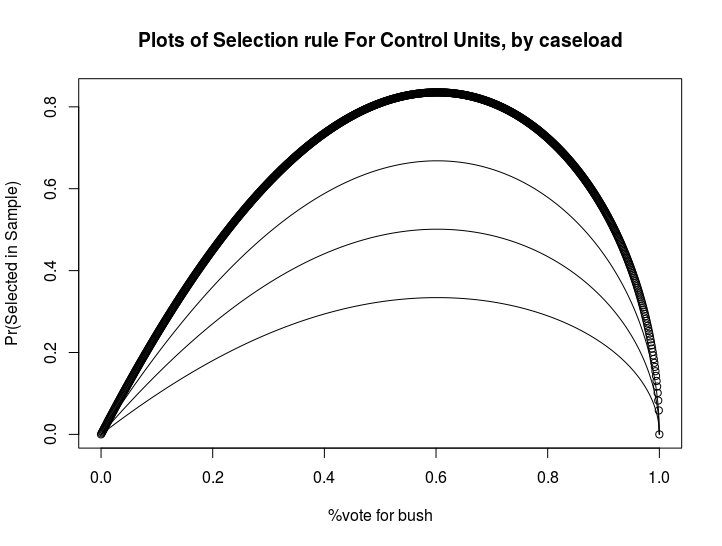
\includegraphics[scale=1]{select_c.png}
\end{sidewaysfigure}

\begin{sidewaysfigure}[!ht]
\label{dc}
\center
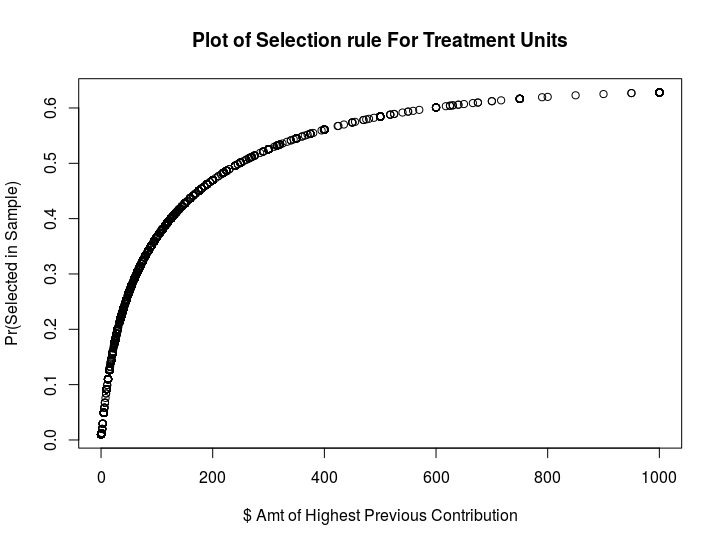
\includegraphics[scale=1]{select_t.png}
\end{sidewaysfigure}

\begin{sidewaysfigure}[!ht]
\label{ps}
\center
\caption{Histogram of propensity scores}
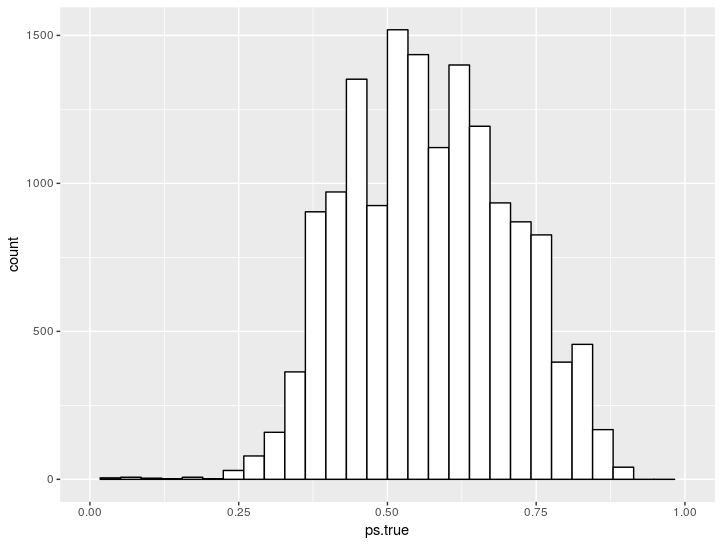
\includegraphics[scale=1]{pscores.png}
\end{sidewaysfigure}

\begin{sidewaysfigure}[!ht]
\label{ol}
\center
\caption{Propensity Score Overlap by Treatment Group}
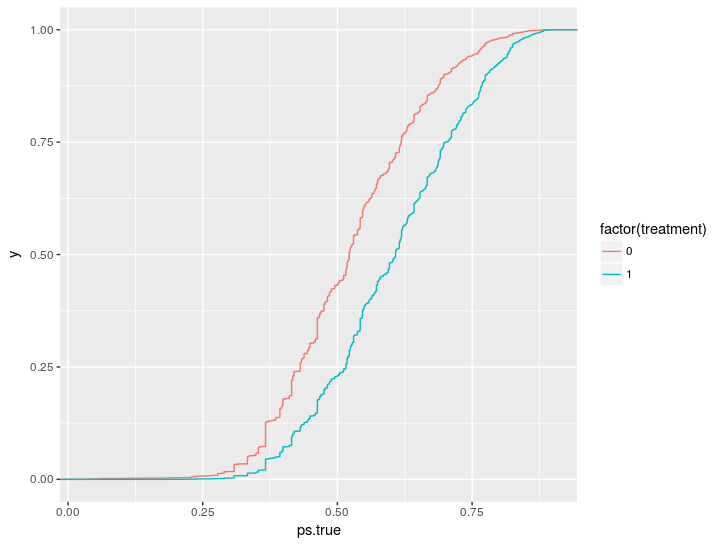
\includegraphics[scale=1]{overlap.png}
\end{sidewaysfigure}

\begin{sidewaysfigure}[!ht]
\label{bias}
\center
\caption{Distribution of bias functions}
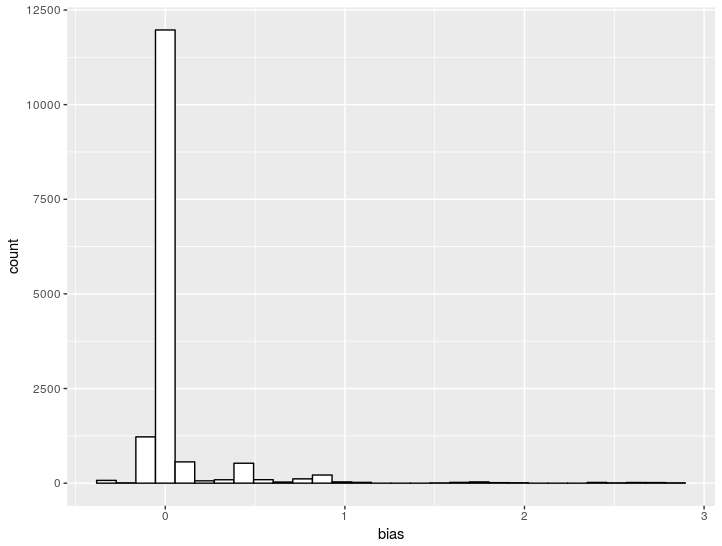
\includegraphics[scale=1]{bias.png}
\end{sidewaysfigure}

\begin{sidewaysfigure}[!ht]
\label{pscores}
\center
\caption{Estimated Propensity Scores and True Propensity Score}
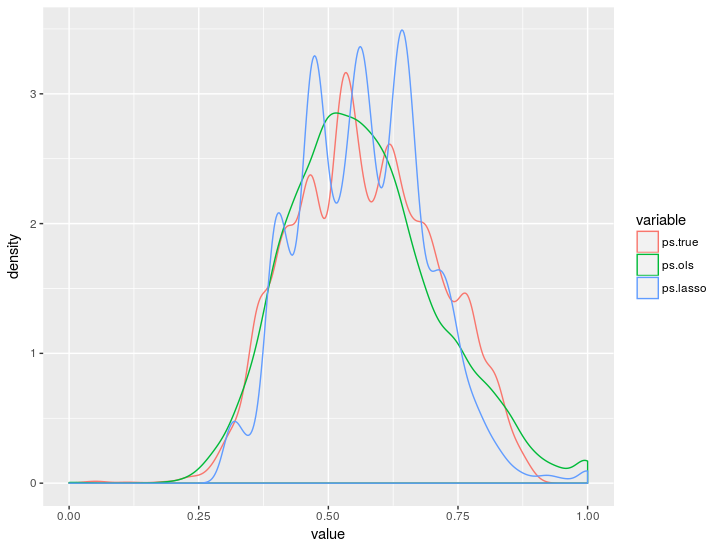
\includegraphics[scale=1]{pscore_ests.png}
\end{sidewaysfigure}

\end{document}